\chapter{Introducción a la filosofía de la ciencia}
\label{cha:filosofiaciencia}

Estás en una carrera de Ciencias, rodeado de Científicos que hacen cosas
científicas, pero ¿qué es exactamente la ciencia?
¿Por qué la astronomía es una ciencia pero la astrología no?
¿A qué se dedican los científicos?
¿Es el método científico la única forma de hacer ciencia?
¿Un conocimiento científico es más confiable que un conocimiento no científico?
Todas estas preguntas son las que discuten los filósofos de la ciencia, y tratar
de responderlas y debatirlas nos brinda un mejor panorama de la naturaleza misma
de esta disciplina.

\section{Los orígenes de la ciencia}
\label{sec:losorigenesdelaciencia}

Para ponernos en contexto es importante conocer los orígenes de la ciencia, así
será más fácil entender por qué funciona como en la actualidad.

\subsection*{La ciencia en la antigüedad}
\label{sub:cienciaenlaantiguedad}
Desde la antigua Grecia, los filósofos se preguntaban por las causas del mundo.
Tal es el caso de \index{Aristóteles}{Aristóteles} (384--322 a. C.), quien
propuso muchas teorías físicas basándose en acertijos conceptuales y
razonamientos lógicos, pero sin experimentación ni
observación\cite{sep-aristotle}.
Es por ello que sus teorías no fueron muy acertadas; por ejemplo, creía que los
cuerpos están compuestos de cuatro elementos: tierra, agua, aire y fuego.
A esta cosmovisión se le conoce como \terminology[aristotelismo]{aristotelismo},
y fue la base de la ciencia hasta el siglo \textsc{xvii}.

Parte central del aristotelismo fue la
\terminology[teoría!geocéntrica]{teoría geocéntrica}, introducida por
\index{Ptolomeo}{Ptolomeo} (90--168 d. C.), Esta postula que la Tierra es el
centro del universo y que todos los demás cuerpos celestes giran alrededor de
ella.

\subsection*{La edad media y el primer científico moderno}
\label{sub:laedadmediayelprimercientificomoderno}
Fue hasta 1542 cuando \index{Copérnico, Nicolás}{Nicolás Copérnico} (1473--1543)
se atrevió a desafiarla publicando su libro \textit{De revolutionibus
    orbium coelestium} (Sobre las revoluciones de las esferas celestes), en el
que propone que el Sol está fijo en el centro del universo y que los planetas
giran alrededor de él, dando lugar así a la
\terminology[teoría!heliocéntrica]{teoría heliocéntrica}.

\begin{figure}[ht]
    \centering
    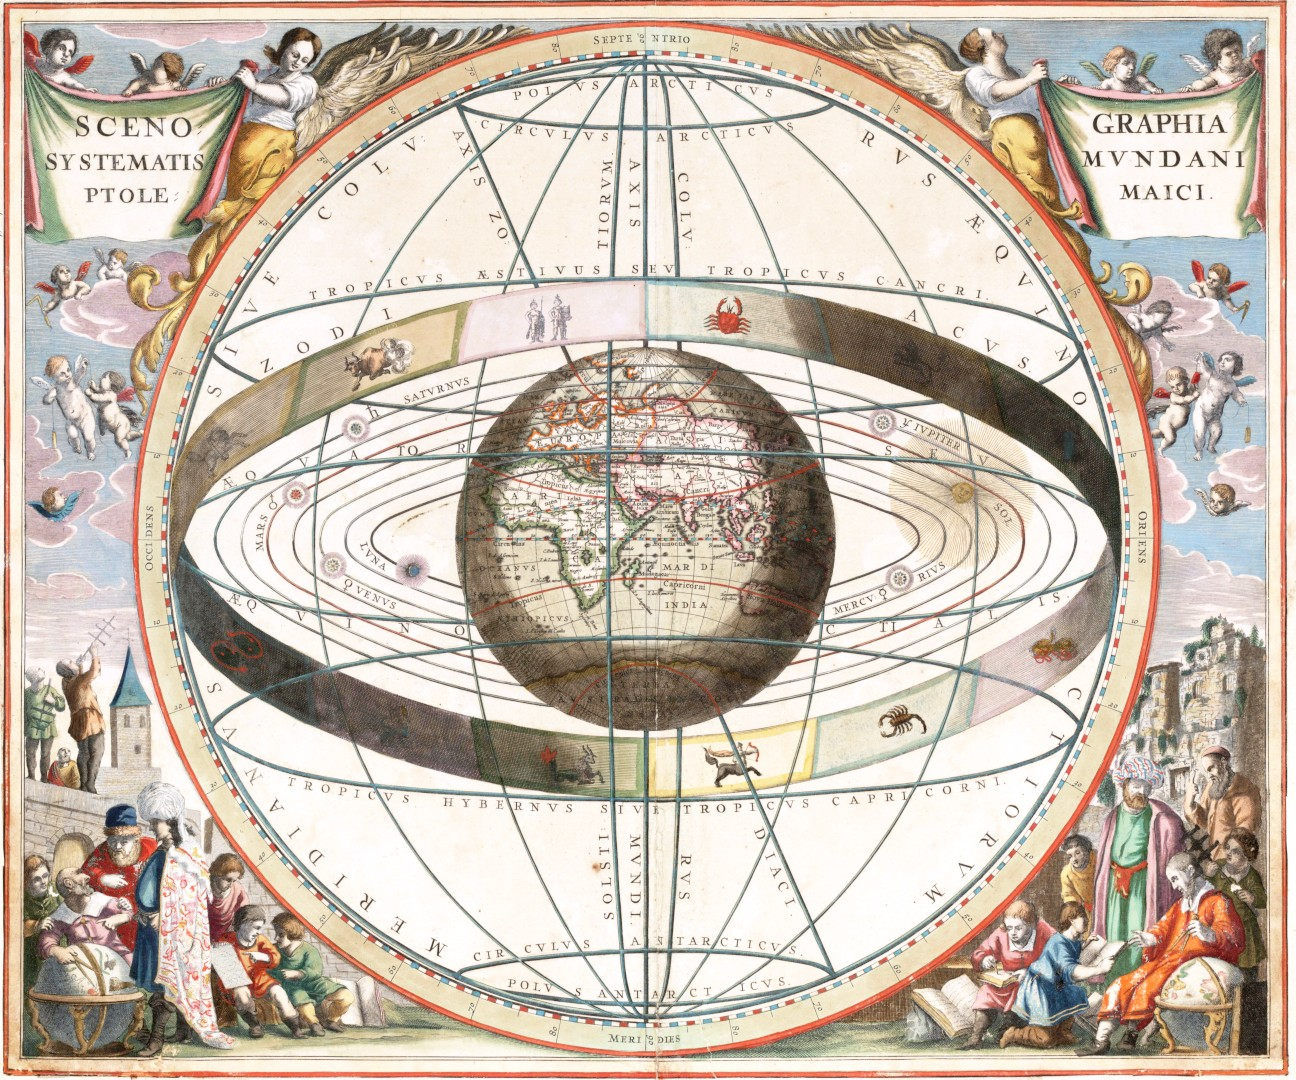
\includegraphics[width=0.8\linewidth]{img/Cellarius_ptolemaic_system}
    \caption{El sistema ptolemaico, en el que la Tierra es el centro del
        universo. Crédito: Loon, J. van (Johannes), aprox. 1611--1686.}
    \label{fig:ptolemaico}
\end{figure}

La teoría no fue bien recibida por la Iglesia, ni aún cuando su autor la dedicó
al Papa Pablo \textsc{iii}.
Más bien fue vetada de 1616 a 1835, pero en solo cien años se había convertido
en la teoría dominante gracias a los trabajos de \index{Galileo Galilei}{Galileo
    Galilei} (1564--1642) y \index{Johannes Kepler}{Johannes Kepler}
(1571--1630).
Kepler descubrió que los planetas se mueven en órbitas elípticas y no circulares
como creía Copérnico, y así resolvió el problema de la posición de Marte en el
cielo nocturno.
En cambio, Galileo apuntó su telescopio al cielo y descubrió que Júpiter tiene
cuatro lunas, que la Luna tiene montañas y cráteres, y que el Sol tiene manchas
entre otras cosas.

Galileo también hizo importantes contribuciones en otras áreas de la ciencia;
descubrió la \emph{ley de caída de los cuerpos}, que dice que todos los cuerpos
caen con la misma aceleración, contradiciendo así a la teoría aristotélica de
que los cuerpos caen con una velocidad proporcional a su peso.
Según relata su discípulo Vivianni esto lo demostró dejando caer dos bolas de
diferente peso desde lo alto de la Torre inclinada de Pisa
\cite{Viviani+2019+1+94}.
Hasta entonces la lógica aristotélica era suficiente para explicar el mundo, la
experimentación era considerada una actividad de segunda clase, y las
matemáticas servían para describir objetos ideales pero no la realidad.
Galileo cambió todo esto, y por ello se le considera el primer científico
moderno.
Desafortunadamente, Galileo fue condenado por la Inquisición en 1633 por
defender a la teoría heliocéntrica, que para entonces era considerada herética
porque contradice la creación del mundo descrita en la Biblia.
Él pasó el resto de su vida bajo arresto domiciliario y se convirtió así también
en el ejemplo más famoso del conflicto entre ciencia y religión.

\subsection*{La revolución científica}
\label{sub:larevolucioncientifica}



\section{Qué es la Ciencia}
\label{sec:queeslaciencia}

La ciencia intenta explicar, entender y predecir el mundo que nos rodea, pero
también la religión, la astrología, e incluso otras disciplinas académicas como
la historia y la filosofía.
La diferencia crucial está en los métodos, a saber: la experimentación,
observación y construcción de teorías; pero esto no fue siempre así, por lo que
es importante ponernos en contexto mediante un breve recorrido histórico antes
de poder delimitar el concepto de ciencia.

\section{Los métodos científicos}
\label{sec:losmetodoscientificos}

\section{Las revoluciones científicas}
\label{sec:lasrevolucionescientificas}

\section{Crítica a la ciencia}
\label{sec:criticaalaciencia}
